\documentclass[handout]{beamer}
\usepackage{multicol}
\usepackage{xy}
\everymath{\displaystyle}
\mode<presentation>
{\usetheme{Warsaw}\setbeamercovered{dynamic}}
\usecolortheme{crane}
\usepackage{beamerfoils}
\pgfdeclareimage[height=1in]{university-logo}{ISULogo}
\logo{\pgfuseimage{university-logo}}
\setbeamertemplate{navigation symbols}{}
\title[\S6]{Section 6\\{\em And} and {\em or} problems}
\author{Dr Marcus Bishop}
\subject{Math 104}
\beamerdefaultoverlayspecification{<+->}
\theoremstyle{definition}
\newtheorem{remark}{Remark}
\newtheorem{impact}{Impact}
\newtheorem{notation}{Notation}
\newtheorem{argument}{Argument}
\usepackage{arev}
\begin{document}
\begin{frame}\titlepage\end{frame}
\LogoOff

\begin{frame}{Card problem from exam}
\begin{itemize}
\item How many cards either are picture cards or have
suit \alert{$\varheart$}?
\item Observe that thirteen cards have
suit \alert{$\varheart$}, namely
\[A\alert{\varheart},
2\alert{\varheart},
3\alert{\varheart},\ldots,
10\alert{\varheart},
J\alert{\varheart},
Q\alert{\varheart},
K\alert{\varheart}\]
\item Observe that twelve cards are picture cards, namely
\[J\alert{\varheart},J\alert{\vardiamond},J\clubsuit,J\spadesuit,
Q\alert{\varheart},Q\alert{\vardiamond},Q\clubsuit,Q\spadesuit,
K\alert{\varheart},K\alert{\vardiamond},K\clubsuit,K\spadesuit\]
\item However, \alert{three} cards in both groups,
namely
\[J\alert{\varheart},Q\alert{\varheart},K\alert{\varheart}\]
\item Thus $13+12-3=22$ cards are either picture cards or have 
suit \alert{$\varheart$}
\end{itemize}
\end{frame}

\begin{frame}{Inclusion-Exclusion Formula}
\begin{theorem}[Inclusion-Exclusion Formula]
Suppose that
\begin{itemize}
\item $M$ has $m$ elements 
\item $N$ has $n$ elements
\item There are $p$ elements in \alert{both} $M$ and $N$
\end{itemize}
Then there are $m+n-p$ elements in \alert{either} $M$ or $N$
\end{theorem}
\end{frame}

\begin{frame}{Example}
\begin{itemize}
\item How many of $1,2,\ldots,12$ are
either divisible by $3$ or greater than $6$?
\item Numbers divisible by $3$: $3,6,9,12$
\item Numbers greater than $6$: $7,8,9,10,11,12$
\item Numbers in both groups: $9,12$
\item Thus $4+6-2=8$
either divisible by $3$ or greater than $6$?
\end{itemize}
\end{frame}

\begin{frame}{Venn diagrams}
\begin{itemize}
\item Can visualize last example using Venn diagram:
\[\begin{xy}<1cm,0cm>:
(-1,0)*\cir<2cm>{};
(1,0)*\cir<2cm>{};
(-1.5,1)*{3};
(-1.5,-1)*{6};
(0,1)*{9};
(0,-1)*{12};
(1.25,1)*{7};
(1.25,-1)*{10};
(2,1)*{8};
(2,-1)*{11};
\end{xy}\]
\item Numbers divisible by $3$ in left circle
\item Numbers greater than $6$ in right circle
\item Numbers in both groups in both circles
\end{itemize}
\end{frame}

\begin{frame}{Greek, Roman, Russian alphabets}
\begin{multicols}{2}
\begin{itemize}
\item Upper left circle shows letters of Greek alphabet
\item Upper right circle shows letters of Roman alphabet
\item Lower circle shows letters of Russian alphabet
\item How many in Roman and Russian but not Greek?
\only<+->{One, namely C}
\item How many letters in all three?
\only<+->{11}
\end{itemize}
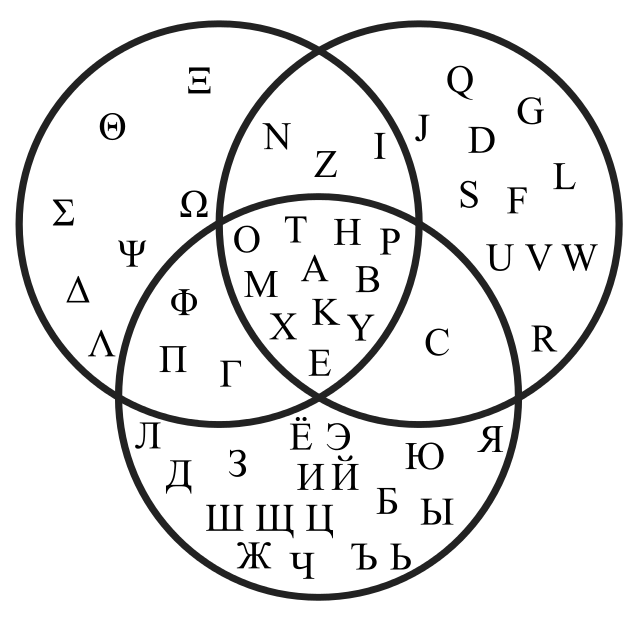
\includegraphics[scale=.25]{Venn}
\end{multicols}
\end{frame}

\begin{frame}{Freshman music majors}
\begin{itemize}
\item $100$ freshman majoring in (instrumental) music
required to be in either band or orchestra
\item $75$ in band
\item $35$ in both band and orchestra
\item How many in orchestra?
\item Rather than drawing freshmen in circles,
write only \alert{number} of freshman in each
group in corresponding region 
\[\begin{xy}<1cm,0cm>:
(-1,2)*+!D{\text{Band}};
(1,2)*+!D{\text{Orch}};
(-1,0)*\cir<2cm>{};
(1,0)*\cir<2cm>{};
(0,0)*{35};
\end{xy}\]
\end{itemize}
\end{frame}

\begin{frame}
\begin{itemize}
\item Since $75$ in band, must have
$40$ in band but not orchestra:
\[\begin{xy}<1cm,0cm>:
(-1,2)*+!D{\text{Band}};
(1,2)*+!D{\text{Orch}};
(-1,0)*\cir<2cm>{};
(1,0)*\cir<2cm>{};
(0,0)*{35};
(-2,0)*{40};
\end{xy}\]
\end{itemize}
\end{frame}

\begin{frame}
\begin{itemize}
\item Must be $100-75=25$ in orchestra but not band:
\[\begin{xy}<1cm,0cm>:
(-1,2)*+!D{\text{Band}};
(1,2)*+!D{\text{Orch}};
(-1,0)*\cir<2cm>{};
(1,0)*\cir<2cm>{};
(0,0)*{35};
(-2,0)*{40};
(2,0)*{25};
\end{xy}\]
\item Thus $35+25=60$ in orchestra
\end{itemize}
\begin{remark}
Solving Inclusion Exclusion Formula
\[75+n-35=100\]
for $n$ obviates Venn diagram
\end{remark}
\end{frame}

\begin{frame}{More Inclusion-Exclusion}
\begin{theorem}[Inclusion-Exclusion Formula]
If $E,F$ events and
\begin{itemize}
\item $p=P\left(E\right)$
\item $q=P\left(F\right)$
\item $r$ the probability that \alert{both} $E$ and $F$ occur
\end{itemize}
then $p+q-r$ the probability that \alert{either} $E$ or $F$ occurs
\end{theorem}
\begin{example}[Exercise 11]
\begin{itemize}
\item Suppose $P\left(E\right)=0.8$,
$P\left(F\right)=0.4$, and $P\left(\text{$E$ and $F$}\right)=0.5$
\item Then $P\left(\text{$E$ or $F$}\right)
=0.8+0.4-0.5=0.7$
\item Example doesn't even require context
\end{itemize}
\end{example}
\end{frame}

\begin{frame}{Example}
\begin{itemize}
\item Recall that $3,6,9,12$ divisible by $3$
\item So if number randomly selected from
$1,2,\ldots,12$ then $4/12$
the probability number divisible by $3$
\item Similarly $7,8,9,10,11,12$ greater than $6$
\item So $6/12$ the probability number
greater than $6$
\item Finally, $9,12$ divisible by $3$ \alert{and}
greater than $6$
\item So $2/12$ the probability that number
both divisible by $3$ and greater than $6$
\item By Inclusion-Exclusion
\[\frac{4}{12}+\frac{6}{12}-\frac{2}{12}=\frac{8}{12}\]
the probability
that number \alert{either} divisible by $3$ or greater than $6$
\item Indeed eight numbers $3,6,7,8,9,10,11,12$ 
divisible by $3$ or greater than $6$
\end{itemize}
\end{frame}

\begin{frame}{Mutually exclusive events}
\begin{itemize}
\item If $0=P\left(\text{$E$ and $F$}\right)$
then $E,F$ called \alert{mutually exclusive events}
\item Means that impossible for \alert{both} $E$ and $F$ to occur
\end{itemize}
\begin{example}
\begin{itemize}
\item Experiment: roll die
\item $E=\left\{1,3,5\right\}$, the event
that odd number rolled
\item $F=\left\{2,4,6\right\}$, the event
that even number rolled
\item Then $E,F$ mutually exclusive
\item Note that as sets, $E,F$ have \alert{no elements} in common
\end{itemize}
\end{example}
\begin{example}
\begin{itemize}
\item But mutually exclusive events need not be \alert{complementary}
\item $E=\left\{1,3,5\right\}$ and $F=\left\{2\right\}$
mutually exclusive
\end{itemize}
\end{example}
\end{frame}

\begin{frame}
\begin{itemize}
\item Note that if $E,F$ mutually exclusive then Inclusion-Exclusion
formula reduces to
\[P\left(\text{$E$ or $F$}\right)=P\left(E\right)
+P\left(F\right)\alert{-0}\]
since $0=P\left(\text{$E$ and $F$}\right)$
\end{itemize}
\begin{example}
\begin{itemize}
\item Experiment: randomly select card
\item $P\left(\clubsuit\right)=\frac{1}{4}=P\left(\alert{\varheart}\right)$
\item $\clubsuit,\alert{\varheart}$ mutually exclusive
since no card has \alert{both} suits
\item Thus $P\left(\text{$\clubsuit$ or $\alert{\varheart}$}\right)
=\frac{1}{4}+\frac{1}{4}=\frac{1}{2}$
\end{itemize}
\end{example}
\end{frame}

\begin{frame}{Independence}
\begin{definition}
$E,F$ called \alert{independent} if $E$
occurring or not has no effect on $F$ occurring or not
\end{definition}
\begin{example}
\begin{itemize}
\item Experiment: flip two coins
\item $E$: first coin lands on heads
\item $F$: second coin lands on heads
\item Then $E,F$ independent
\item Note that 
\[P\left(\text{$E$ and $F$}\right)=P\left(HH\right)
=\frac{1}{4}
=\frac{1}{2}\cdot\frac{1}{2}=P\left(E\right)P\left(F\right)\]
\end{itemize}
\end{example}
\end{frame}

\begin{frame}
\begin{example}
\begin{itemize}
\item Experiment: Draw two cards without replacement
\item $E$: First card has suit $\clubsuit$
\item $F$: Second card has suit $\clubsuit$
\item Then $E,F$ \alert{not} independent!
\item Indeed, $F$ occurring depends on whether or not
$E$ occurred!
\item If $E$ occurs, then $P\left(F\right)=\frac{12}{51}$
since $12$ of remaining $51$ cards have suit $\clubsuit$
\item However if $E$ fails to occur, then $P\left(F\right)=\frac{13}{51}$
since $13$ of remaining $51$ cards have suit $\clubsuit$
\end{itemize}
\end{example}
\end{frame}

\begin{frame}{Independence and \em{and}}
\begin{theorem}
If $E,F$ independent, then
$P\left(\text{$E$ and $F$}\right)=P\left(E\right)P\left(F\right)$
\end{theorem}
\begin{example}
\begin{itemize}
\item Suppose family plans to have two children
\item Calculate probability that both children girls
\item $E_1=\left\{\text{first child girl}\right\}$
\item $E_2=\left\{\text{second child girl}\right\}$
\item Then $E_1,E_2$ independent
\item $P\left(E_1\right)=1/2=P\left(E_2\right)$ so
\end{itemize}
\only<+->{
\begin{multline*}
P\left\{\text{both children girls}\right\}
\only<+->{=P\left(\text{$E_1$ and $E_2$}\right)\\}
\only<+->{=P\left(E_1\right)P\left(E_2\right)}
\only<+->{=\frac{1}{2}\cdot\frac{1}{2}}
\only<+->{=\frac{1}{4}}
\end{multline*}}
\end{example}
\end{frame}

\begin{frame}{Children continued}
\begin{itemize}
\item Suppose family plans to have \alert{ten} children
\item Calculate probability that all ten children girls
\item $E_1=\left\{\text{first child girl}\right\},\ldots,
E_{10}=\left\{\text{tenth child girl}\right\}$
\item Then $E_1,\ldots,E_{10}$ independent
\item $\frac{1}{2}=P\left(E_1\right)=P\left(E_2\right)=\cdots$
\only<+->{
\begin{multline*}
P\left\{\text{all ten children girls}\right\}
\only<+->{=P\left(\text{$E_1$ and $\cdots$ and $E_{10}$}\right)\\}
\only<+->{=P\left(E_1\right)P\left(E_2\right)\cdots P\left(E_{10}\right)}
\only<+->{=\left(\frac{1}{2}\right)^{10}}
\only<+->{=\frac{1}{1024}}
\end{multline*}}
\end{itemize}
\begin{remark}
If they succeed and decide to have another child,
$1/2$ still the probability that eleventh child a girl
\end{remark}
\end{frame}

\begin{frame}{Same problem, different story}
\begin{itemize}
\item You guess on all ten questions of true-false quiz
\item Calculate probability of answering all ten correctly
\item $E_1=\left\{\text{first question correct}\right\},\ldots,
E_{10}=\left\{\text{tenth question correct}\right\}$
\item Then $E_1,\ldots,E_{10}$ independent
and $1/2=P\left(E_1\right)=P\left(E_2\right)=\cdots$
\only<+->{\begin{multline*}
P\left\{\text{all ten questions correct}\right\}
\only<+->{=P\left(\text{$E_1$ and $\cdots$ and $E_{10}$}\right)\\}
\only<+->{=P\left(E_1\right)P\left(E_2\right)\cdots P\left(E_{10}\right)}
\only<+->{=\left(\frac{1}{2}\right)^{10}}
\only<+->{=\frac{1}{1024}}
\end{multline*}}
\item By same argument $\frac{1}{1024}$ also the probability
of answering all questions \alert{incorrectly}
\item So $\frac{1023}{1024}$ the probability of
\alert{not} answering every question incorrectly!
\end{itemize}
\end{frame}

\begin{frame}{Further variation}
\begin{itemize}
\item You guess on all ten questions of multiple choice quiz
\item All ten questions have five choices
\item Calculate probability of answering all ten correctly
\item $\frac{1}{5}=P\left(E_1\right)=P\left(E_2\right)=\cdots$ so
\only<+->{
\begin{multline*}
P\left\{\text{all ten questions correct}\right\}
\only<+->{=P\left(\text{$E_1$ and $\cdots$ and $E_{10}$}\right)\\}
\only<+->{=P\left(E_1\right)P\left(E_2\right)\cdots P\left(E_{10}\right)}
\only<+->{=\left(\frac{1}{5}\right)^{10}}
\only<+->{=\frac{1}{9765625}}
\end{multline*}}
\end{itemize}
\begin{remark}
\begin{itemize}
\item Most people would be happy with seven or eight correct
\item More difficult to compute, see \S11
\end{itemize}
\end{remark}
\end{frame}

\begin{frame}{$\clubsuit$ example revisited}
\begin{itemize}
\item Experiment: Draw two cards without replacement
\item $E$: First card has suit $\clubsuit$
\item $F$: Second card has suit $\clubsuit$
\begin{remark}
\begin{itemize}
\item We interpret \alert{$E$ and $F$} to mean $E$ occurs
\alert{and then} $F$ occurs
\item Thus we assume $E$ has already occurred when considering $F$
\item In this sense, $E,F$ \alert{independent} for purpose of calculating
$P\left(\text{$E$ and $F$}\right)$, so
$P\left(\text{$E$ and $F$}\right)=P\left(E\right)P\left(F\right)$
\end{itemize}
\end{remark}
\item $P\left(E\right)=\frac{13}{52}$
\item $E$ having occurred, $P\left(F\right)=\frac{12}{51}$
\item Thus $P\left(\text{$E$ and $F$}\right)
\only<+->{=\frac{13}{52}\cdot\frac{12}{51}}
\only<+->{=\frac{156}{2652}}\only<+->{=\frac{1}{17}}$
\end{itemize}
\end{frame}

\begin{frame}{Birthday problem}
\begin{itemize}
\item $E$: Two people in room of $24$ have same birthday
\item Calculate $P\left(E\right)$
\item Problem very complicated
\item Simpler to calculate $P\left(\text{not $E$}\right)$
\item That is, calculate probability that all $24$ people
have different birthdays
\item Second person has probability $\frac{364}{365}$ of
not having same birthday as first
\item Third person has probability $\frac{363}{365}$ of
not having same birthday as first or second
\[\frac{364}{365}
\cdot\frac{363}{365}
\cdots\frac{342}{365}\approx 0.462\]
\item So $P\left(E\right)=1-0.462=0.538$ (\alert{!})
\end{itemize}
\end{frame}

\begin{frame}{Summary}
\begin{enumerate}
\item If $E,F$ mutually exclusive then
$P\left(\text{$E$ or $F$}\right)=P\left(E\right)+P\left(F\right)$
\begin{example} $1/4+1/4$ the probability
of drawing $\clubsuit$ or $\alert{\varheart}$ \end{example}
\item If $E,F$ \alert{not} mutually exclusive then
$P\left(\text{$E$ or $F$}\right)=P\left(E\right)+P\left(F\right)
-P\left(\text{$E$ and $F$}\right)$
\begin{example} $1/4+1/13-1/52$ the probability
of drawing $\alert{\varheart}$ or a King\end{example}
\item If $E,F$ independent then
$P\left(\text{$E$ and $F$}\right)=P\left(E\right)P\left(F\right)$
\begin{example} $\left(1/2\right)\left(1/2\right)$ the probability
of both coins landing on heads\end{example}
\end{enumerate}
\end{frame}

%\begin{frame}{Quiz instructions}
%\begin{itemize}
%\item First submit homework \alert{without fringe}
%\item Use number 2 pencil
%\item No phones
%\item Fill in student ID in \alert{first nine spaces},
%leaving tenth space empty
%\item Leave when finished, depositing quiz and answer sheet
%face-down on table in back
%\item Yellow and red forms of quiz in \alert{different piles}
%\end{itemize}
%\end{frame}

\begin{frame}{Two dice}
\begin{itemize}
\item Since rolling die has $6$ outcomes, rolling
two die has $6\cdot 6=36$ outcomes
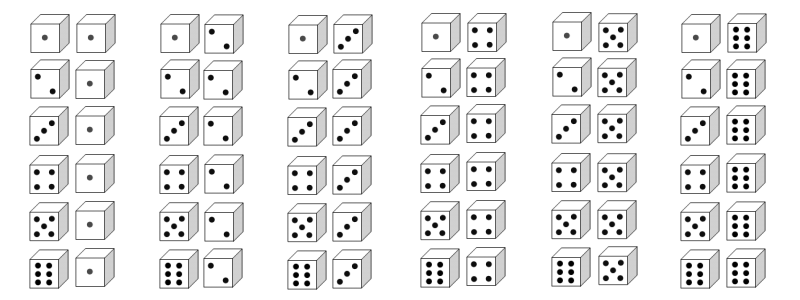
\includegraphics{TwoDice}
\item Rolling two dice and adding has $11$ outcomes,
namely $2,3,\ldots,12$
\item[]
\[\begin{array}{r|c|c|c|c|c|c|c|c|c|c|c}
\text{Sum}&2&3&4&5&6&7&8&9&10&11&12\\\hline
\text{Frequency}&\only<+->{1}&
\only<+->{2}& \only<+->{3}& \only<+->{4}& \only<+->{5}&
\only<+->{6}& \only<+->{5}& \only<+->{4}& \only<+->{3}&
\only<+->{2}& \only<+->{1} \end{array}\]
\end{itemize}
\end{frame}

\begin{frame}{Craps}
\begin{itemize}
\item Each player chooses to be either a \alert{pass bettor}
or a \alert{don't pass bettor}
\item \alert{Shooter} rolls two dice
\item If $7$ or $11$ the sum (a \alert{natural}) then pass bettors win
\item If $2$, $3$, or $12$ the sum (a \alert{craps})
then don't pass bettors win
\item If $4,5,6,8,9,10$ the sum then this number called the \alert{point}
\item Shooter rolls dice until sum is either $7$ or the point
\item If point occurs first, then pass bettors win (\alert{point is made})
\item If $7$ occurs first, then don't pass bettors win
\item Game continues as above, with dice rolled by same shooter
until point established and fails to be made
\end{itemize}
\end{frame}

\begin{frame}
\begin{itemize}
\item Want to calculate expected proceeds for pass bettors
\item Need to enumerate all possible outcomes and find probability of each
\[\begin{xy}<1.4cm,0cm>:
(4.5,0)="0"; (1,-2)="N"; (2,-2)="C"; (3,-2)="4";
(4,-2)="5"; (5,-2)="6"; (6,-2)="8"; (7,-2)="9"; (8,-2)="10";
"0";"N"*+!D{N}**\dir{-};
"0";"C"*+!D{C}**\dir{-};
"0";"4"*+!D{4}**\dir{-};
"0";"5"*+!D{5}**\dir{-};
"0";"6"*+!D{6}**\dir{-};
"0";"8"*+!D{8}**\dir{-};
"0";"9"*+!D{9}**\dir{-};
"0";"10"*+!D{10}**\dir{-};
"4";(2.75,-4)*+!D{P}**\dir{-};
"4";(3.25,-4)*+!D{F}**\dir{-};
"5";(3.75,-4)*+!D{P}**\dir{-};
"5";(4.25,-4)*+!D{F}**\dir{-};
"6";(4.75,-4)*+!D{P}**\dir{-};
"6";(5.25,-4)*+!D{F}**\dir{-};
"8";(5.75,-4)*+!D{P}**\dir{-};
"8";(6.25,-4)*+!D{F}**\dir{-};
"9";(6.75,-4)*+!D{P}**\dir{-};
"9";(7.25,-4)*+!D{F}**\dir{-};
"10";(7.75,-4)*+!D{P}**\dir{-};
"10";(8.25,-4)*+!D{F}**\dir{-};
\end{xy}\]
\end{itemize}
\end{frame}

\begin{frame}
\begin{itemize}
\item $P\left(N\right)=
P\left(\text{$7$ or $11$}\right)
=\frac{6}{36}+\frac{2}{36}=\frac{8}{36}$
since $7$ and $11$ mutually exclusive
\[\begin{xy}<1.4cm,0cm>:
(4.5,0)="0";
(1,-2)="N";(2,-2)="C";(3,-2)="4";(4,-2)="5";
(5,-2)="6";(6,-2)="8";(7,-2)="9";(8,-2)="10";
"0";"N"*+!D{N}**\dir{-}?*+!R{\alert{\frac{8}{36}}};
"0";"C"*+!D{C}**\dir{-};
"0";"4"*+!D{4}**\dir{-};
"0";"5"*+!D{5}**\dir{-};
"0";"6"*+!D{6}**\dir{-};
"0";"8"*+!D{8}**\dir{-};
"0";"9"*+!D{9}**\dir{-};
"0";"10"*+!D{10}**\dir{-};
"4";(2.75,-4)*+!D{P}**\dir{-};
"4";(3.25,-4)*+!D{F}**\dir{-};
"5";(3.75,-4)*+!D{P}**\dir{-};
"5";(4.25,-4)*+!D{F}**\dir{-};
"6";(4.75,-4)*+!D{P}**\dir{-};
"6";(5.25,-4)*+!D{F}**\dir{-};
"8";(5.75,-4)*+!D{P}**\dir{-};
"8";(6.25,-4)*+!D{F}**\dir{-};
"9";(6.75,-4)*+!D{P}**\dir{-};
"9";(7.25,-4)*+!D{F}**\dir{-};
"10";(7.75,-4)*+!D{P}**\dir{-};
"10";(8.25,-4)*+!D{F}**\dir{-};
(1,-4)*+!U{\alert{\frac{2}{9}}};
\end{xy}\]
\end{itemize}
\end{frame}

\begin{frame}
\begin{itemize}
\item Want to calculate $P\left(\text{$4$ and $P$}\right)$
\item $3$ ways to roll $4$ so $P\left(4\right)=\frac{3}{36}$
\item Assume $4$ occurs
\item $3$ ways to roll $4$ again, resulting in $P$
\item $6$ ways to roll $7$, resulting in $F$
\item Outcomes other than $4$ and $7$ ignored
\item So $9$ possible outcomes
\item Thus $P\left(P\right)=\frac{3}{9}$
and $P\left(F\right)=\frac{6}{9}$
\item Therefore
$P\left(\text{$4$ and $P$}\right)
=\frac{3}{36}\cdot\frac{3}{9}=\frac{1}{36}$
\item Similarly $P\left(\text{$4$ and $F$}\right)
=\frac{3}{36}\cdot\frac{6}{9}=\frac{1}{18}$
\end{itemize}
\end{frame}

\begin{frame}
\[\begin{xy}<1.4cm,0cm>:
(4.5,0)="0";
(1,-2)="N";(2,-2)="C";(3,-2)="4";(4,-2)="5";
(5,-2)="6";(6,-2)="8";(7,-2)="9";(8,-2)="10";
"0";"N"*+!D{N}**\dir{-}?*+!R{\frac{8}{36}};
"0";"C"*+!D{C}**\dir{-};
"0";"4"*+!D{4}**\dir{-}?*{\alert{\frac{3}{36}}};
"0";"5"*+!D{5}**\dir{-};
"0";"6"*+!D{6}**\dir{-};
"0";"8"*+!D{8}**\dir{-};
"0";"9"*+!D{9}**\dir{-};
"0";"10"*+!D{10}**\dir{-};
"4";(2.75,-4)*+!D{P}**\dir{-}?*{\alert{\frac{3}{9}}};
"4";(3.25,-4)*+!D{F}**\dir{-}?*{\alert{\frac{6}{9}}};
"5";(3.75,-4)*+!D{P}**\dir{-};
"5";(4.25,-4)*+!D{F}**\dir{-};
"6";(4.75,-4)*+!D{P}**\dir{-};
"6";(5.25,-4)*+!D{F}**\dir{-};
"8";(5.75,-4)*+!D{P}**\dir{-};
"8";(6.25,-4)*+!D{F}**\dir{-};
"9";(6.75,-4)*+!D{P}**\dir{-};
"9";(7.25,-4)*+!D{F}**\dir{-};
"10";(7.75,-4)*+!D{P}**\dir{-};
"10";(8.25,-4)*+!D{F}**\dir{-};
(1,-4)*+!U{\frac{2}{9}};
(2.75,-4)*+!U{\alert{\frac{1}{36}}};
(3.25,-4)*+!U{\alert{\frac{1}{18}}};
\end{xy}\]
\end{frame}

\begin{frame}{Homework for Monday 6 October}
\begin{itemize}
\item Print or otherwise reproduce slide 28
\item Calculate probability of remaining outcomes,
writing them directly on tree
\item Verify that $1$ the sum of probabilities
of all outcomes
\item Assuming that pass bettors and
don't pass bettors each bet $100$,
calculate expected proceeds for both groups.
\item Also complete exercises 15--34 of textbook
\end{itemize}
\end{frame}

\begin{frame}{Probabilities of all winning outcomes}
\begin{itemize}
\item $P\left(N\right)=2/9$ (calculation above)
\item $P\left(\text{$4$ and $P$}\right)=1/36$ (calculation above)
\item $P\left(\text{$5$ and $P$}\right)=\frac{4}{36}\cdot\frac{4}{10}
=\frac{2}{45}$
\item $P\left(\text{$6$ and $P$}\right)=25/396$
\item $P\left(\text{$8$ and $P$}\right)=25/396$
\item $P\left(\text{$9$ and $P$}\right)=2/45$
\item $P\left(\text{$10$ and $P$}\right)=1/36$
\item So pass bettors win $\$100$ with probability
\[\frac{2}{9}+2\left(\frac{1}{36}\right)
+2\left(\frac{2}{45}\right)+2\left(\frac{25}{396}\right)
=\frac{244}{495}\approx 0.4929\]
\end{itemize}
\end{frame}

\begin{frame}{Probabilities of all losing outcomes}
\begin{itemize}
\item $P\left(C\right)=\frac{4}{36}=\frac{1}{9}$
\item $P\left(\text{$4$ and $F$}\right)=1/18$ (calculation above)
\item $P\left(\text{$5$ and $F$}\right)=\frac{4}{36}\cdot\frac{6}{10}
=\frac{1}{15}$
\item $P\left(\text{$6$ and $F$}\right)=5/66$
\item $P\left(\text{$8$ and $F$}\right)=5/66$
\item $P\left(\text{$9$ and $F$}\right)=1/15$
\item $P\left(\text{$10$ and $F$}\right)=1/18$
\item So pass bettors lose $\$100$ with probability
\[\frac{1}{9}+2\left(\frac{1}{18}\right)
+2\left(\frac{1}{15}\right)+2\left(\frac{5}{66}\right)
=\frac{251}{495}\approx 0.507\]
\end{itemize}
\end{frame}

\begin{frame}{Craps expectation}
\begin{itemize}
\item Observe that $\frac{244}{495}+\frac{251}{495}=1$
\item Expected proceeds for pass bettors:
\[100\left(\frac{244}{495}\right)-100\left(\frac{251}{495}\right)
=-\frac{140}{99}\approx \$-1.41\]
\item Expected proceeds for don't pass bettors:
\[-100\left(\frac{244}{495}\right)+100\left(\frac{251}{495}\right)
=\frac{140}{99}\approx \$1.41\]
\end{itemize}
\end{frame}

\begin{frame}{Casino craps}
\begin{itemize}
\item In casino, payouts for pass bettors the same as in street version
\item So pass bettors win amount bet
for favorable outcomes: $N$,
$\left(\text{$4$ and $P$}\right)$,\dots,
$\left(\text{$12$ and $P$}\right)$
\item Thus $\$-1.41$ the expectation for pass bettors
for every $\$100$ bet
\item However, if initial roll results in $12$, don't pass bettors
neither win nor lose
\item Thus outcome $C$ splits into two outcomes for don't pass bettors:
\begin{itemize}
\item Don't pass bettors win amount bet if first roll $2$ or $3$
\item Don't pass bettors win $0$ if first roll $12$
\end{itemize}
\end{itemize}
\end{frame}

\begin{frame}
\begin{itemize}
\item Recall that expected proceeds for don't pass bettors
in \alert{street} version:
\[-100\left(\frac{244}{495}\right)+100\left(\alert{\frac{251}{495}}\right)
=\frac{140}{99}\approx \$1.41\]
\item Here
\[\frac{251}{495}
=\alert{\frac{1}{9}}+2\left(\frac{1}{18}\right)
+2\left(\frac{1}{15}\right)+2\left(\frac{5}{66}\right)\]
\item Here $\frac{1}{9}=\frac{4}{36}$ the probability of $C$
\item In \alert{casino} version, change $\frac{1}{9}$ to
$\frac{3}{36}=\frac{1}{12}$, the probability of $2$ or $3$
\end{itemize}
\end{frame}

\begin{frame}
\begin{itemize}
\item Thus outcome $\$100$ occurs with probability
\[\alert{\frac{1}{12}}+2\left(\frac{1}{18}\right)
+2\left(\frac{1}{15}\right)+2\left(\frac{5}{66}\right)
=\frac{949}{1980}\approx 0.4793\]
\item Thus expectation for don't pass bettors
\[-100\left(\frac{244}{495}\right)+100\left(\alert{\frac{949}{1980}}\right)
+\alert{0\left(\frac{1}{36}\right)}
=-\frac{15}{11}\approx \$-1.37\]
\item Thus expectation for pass bettors $\$-1.41$
close to expectation for don't pass bettors
\end{itemize}
\end{frame}

\begin{frame}{Chuck-a-luck}
\begin{multicols}{2}
\begin{itemize}
\item Chuck-a-luck popular in carnivals, less
popular in casinos
\item Played with three regular dice
\item Players bet on one of $1,2,\ldots,6$
\item Dealer rolls three dice
\item House pays player amount bet for every
die showing chosen number
\item However, if no die shows chosen number,
house keeps bet
\end{itemize}
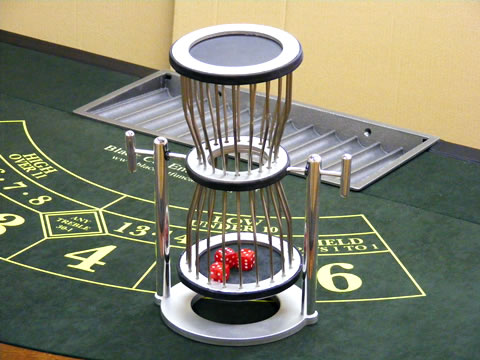
\includegraphics[scale=.35]{Chuck}
\end{multicols}
\end{frame}

\begin{frame}
\begin{example}
\begin{itemize}
\item Suppose player bets $\$1$ on number $3$
\item If dice show $3,1,6$ player wins $\$1$
\item If dice show $1,3,3$ player wins $\$2$
\item If dice show $1,5,2$ player loses $\$1$
\end{itemize}
\end{example}
\begin{center}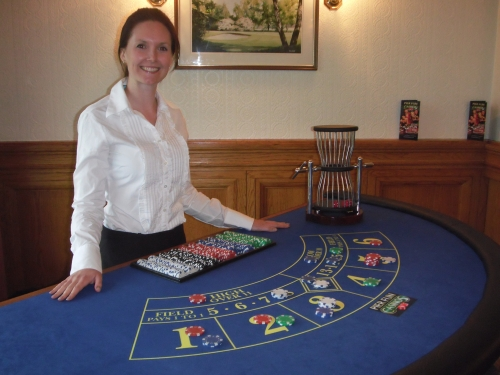
\includegraphics[scale=.35]{Chuck2}\end{center}
\end{frame}

\begin{frame}
Chuck-a-luck seems attractive by following \alert{incorrect} argument
\begin{argument}
\begin{itemize}
\item Suppose $1$ the chosen number (for concreteness)
\item Let $E_1$ be event that first die shows $1$
\item Let $E_2,E_3$ be events that second, third dice show $1$
\item Then $P\left(E_1\right)=P\left(E_2\right)=P\left(E_3\right)
=\frac{1}{6}$
\item So $P\left(\text{$E_1$ or $E_2$ or $E_3$}\right)
=\frac{1}{6}+\frac{1}{6}+\frac{1}{6}=\frac{1}{2}$
the probability that at least one die shows $1$
\item Thus game is at least fair
\item Furthermore, possibility of \alert{multiple} dice
showing $1$ further increases chances of winning
\end{itemize}
\end{argument}
But $E_1,E_2,E_3$ \alert{not mutually exclusive}!
\end{frame}

\begin{frame}{Chuck-a-luck probabilities}
\begin{itemize}
\item $216=6^3$ the number of possible outcomes
\item $1,1,1$ occurs in only one way, so $\frac{1}{216}$
the probability of $1,1,1$
\item Two $1$'s occurs in five ways as $1,1,x$
where $x\ne 1$
\item Can also occur in further five ways as $1,x,1$
and still further five ways as $x,1,1$
\item So $\frac{15}{216}$ the probability of two $1$'s
\item Single $1$ occurs as $1,x,y$ where $x,y\ne 1$
\item Occurs in $5\cdot 5=25$ ways
\item Single $1$ occurs in further $25$ ways as $x,1,y$
and still further $25$ ways as $x,y,1$
\item Thus $\frac{75}{216}$ the probability of single $1$
\end{itemize}
\end{frame}

\begin{frame}
\begin{itemize}
\item Note that $\frac{1}{216}+\frac{15}{216}+\frac{75}{216}
=\frac{91}{216}\approx 0.4213$ the probability of winning
\item Note that $0.4213<0.5$ so Chuck-a-luck \alert{not} fair!
\item Note that $1-\frac{91}{216}=\frac{125}{216}$
the probability of losing
\item If player bets $\$1$ then expectation
\begin{multline*}
3\left(\frac{1}{216}\right)
+2\left(\frac{15}{216}\right)+1\left(\frac{75}{216}\right)
-1\left(\frac{125}{216}\right)\\
=-\frac{17}{216}\approx \$-0.0787
\end{multline*}
\item So player expected to lose $7.87$ cents per dollar spent
in long run
\end{itemize}
\end{frame}

\begin{frame}{Exam instructions}
\begin{itemize}
\item Don't email ungraded homework to Fatema
\item In case of incorrect grade entry, email
a photo or scan of homework to Fatema at {\texttt faftab@iastate.edu}
\item Write your name
\item No phones
\item You \alert{may} use calculator
\item Unjustified correct answers make you look suspicious:
\alert{show work}!
\item Please ask for clarification in case of confusion
\item We will provide scratch paper if needed
\item Don't use your own paper
\item When finished exit in back, placing exam on table
\item Submit scratch paper also
\end{itemize}
\end{frame}

\end{document}
